\section[Arbres de Décision pour la classification]{Arbres de Décision pour la classification}

\subsection[Algorithme CART]{Algorithme CART}

\begin{frame}{Problème mono-dimensionnel et linéairement séparable}
	\begin{figure}
		\centering
		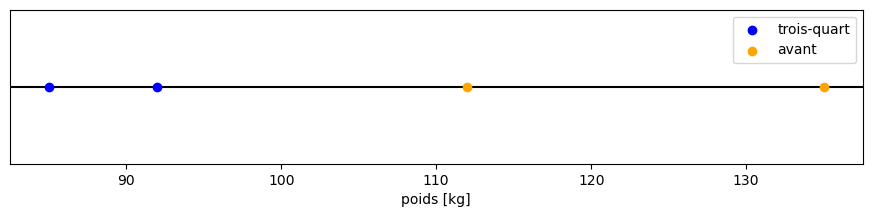
\includegraphics[width=0.85\linewidth]{Images/lineairement_separable_1}
		\label{fig:lineairement_separable_1}
	\end{figure}				
	Dans l'exemple ci-dessus on cherche à classer les joueurs de rugby selon leur poids. Ce problème est linéairement séparable: il existe au moins une valeur de poids qui permet de \textbf{parfaitement} séparer les avants des trois-quarts.
	
	\pause
	\vspace{0.5cm}
	L'idée consiste à choisir un poids qui sépare les données en deux groupes de sorte que la somme pondérée des \textbf{entropies} des groupes soit \textbf{minimale}.
	
	\pause
	\vspace{0.5cm}
	C'est le principe de fonctionnement de l'algorithme \textbf{CART}: Classification And Regression Trees.
	
\end{frame}

\begin{frame}{Problème mono-dimensionnel et linéairement séparable}
	Pour un poids de séparation donné, l'entropie se calcule comme:
	\begin{align*}
		H(P) &= P(X = \text{"trois-quart"}) I(X = \text{"trois-quart"}) \\
		&\quad + P(X = \text{"avant"}) I(X = \text{"avant"}) \\
		&= - P(X = \text{"trois-quart"}) \ln P(X = \text{"trois-quart"}) \\
		&\quad - P(X = \text{"avant"}) \ln P(X = \text{"avant"})
	\end{align*}
	Considérons les options suivantes:
	\begin{itemize}
		\item Poids de séparation: 90 kilogrammes
		\begin{itemize}
			\item Dans le groupe de gauche: 1 trois-quart. $H_{\text{gauche}} \to 0$.
			\item Dans le groupe de droite: 1 trois-quart et 2 avants: $H_{\text{droite}} = - \frac{1}{3} \ln \frac{1}{3} - \frac{2}{3} \ln \frac{2}{3} \approx 0.64$
		\end{itemize}
		\pause
		\item Poids de séparation: 100 kilogrammes
		\begin{itemize}
			\item Dans le groupe de gauche: 2 trois-quart. $H_{\text{gauche}} \to 0$.
			\item Dans le groupe de droite: 2 avants: $H_{\text{droite}} \to 0$.
		\end{itemize}		
	\end{itemize}
	\pause
	On retient donc une valeur de séparation de poids de 100 kilogrammes puisque la somme des entropies est nulle.
\end{frame}

\begin{frame}{Algorithme pour un problème mono-dimensionnel}
	Pour les données d'apprentissage $X \in \mathcal{X}$ avec $\mathcal{X} \subset \R$ et $Y \in\{0, 1\}$:
	\begin{enumerate}
		\item On trie les données d'apprentissage $\mathcal{D} = \{(x^{(i)}, y^{(i)})\}_{i=1}^n$ par valeur croissante de $x$.
		\pause
		\item Pour chaque $k \in \llbracket 2; n \rrbracket$, on évalue une valeur de séparation $x^* = \left(x_{(k)} + x_{(k - 1)}\right) / 2$ où $x_{(k)}$ représente l'observation $x$ au rang $k$. $x^*$ est le point médian.
		\begin{itemize}
			\item On calcule l'entropie dans le groupe (\textbf{branche}) de gauche: $\{(x, y) \in \mathcal{D} \mid x < x^*\}$.
			\item On calcule l'entropie dans le groupe de droite: $\{(x, y) \in \mathcal{D} \mid x > x^*\}$.
			\item On calcule la somme des deux entropies pondérée par le nombre d'observations dans chaque groupe.
		\end{itemize}
		\pause
		\item On retient la valeur de $x^*$ qui minimise cette somme pondérée.
	\end{enumerate}
\end{frame}

\begin{frame}{Algorithme pour un problème multi-dimensionnel}
	Pour les données d'apprentissage $X \in \mathcal{X}$ avec $\mathcal{X} \subset \R^d$ et $Y \in\{0, 1\}$:
	\begin{enumerate}
		\item Pour chaque $j \in \llbracket 1; d \rrbracket$ on applique l'algorithme du problème mono-dimensionnel en considérant uniquement la caractéristique $X_j$.
		\begin{itemize}
			\item On obtient donc une somme pondérée pour chaque valeur de $j$.
			\item Chaque somme pondérée est associée à une valeur de séparation $x_j^*$ optimale.
		\end{itemize}
		\pause
		\item On retient la valeur de $j$ pour laquelle la somme pondérée des entropies est minimale et la valeur de séparation associée $x_j^*$.
		\pause
		\item On sépare les observations en deux groupes:
		\begin{itemize}
			\item Gauche: $\{(x, y) \in \mathcal{D} \mid x_j < x_j^*\}$.
			\item Droite: $\{(x, y) \in \mathcal{D} \mid x_j > x_j^*\}$.
		\end{itemize}
		\pause
		\item \`A chaque groupe on assigne une profondeur de 1.
	\end{enumerate}
\end{frame}

\begin{frame}{Algorithme récursif}
	L'algorithme est récursif. On ré-applique donc l'algorithme du problème multi-dimensionnel à chaque groupe ainsi créé.
	\begin{enumerate}
		\item Pour chaque groupe créé précédemment on vérifie un critère d'arrêt:
			\begin{itemize}
				\item Si la profondeur du groupe atteint une valeur maximum fixée, on s'arrête. La profondeur représente le nombre de découpes récursives depuis les données initiales (le nombre maximum de \textbf{ramifications}).
				\item Si l'entropie du groupe atteint une valeur minimum fixée, on s'arrête.
				\item Si la taille du groupe atteint un nombre d'observations minimum fixé, on s'arrête.
			\end{itemize}
		\item Si un critère d'arrêt est trouvé, on associe à ce groupe la proportion d'observations pour lesquelles $Y = 1$. C'est cette valeur qui nous permettra de faire une prédiction plus tard.
		\item Si aucun critère d'arrêt n'est rencontré, on sépare le groupe parent en deux nouveaux groupes enfants en suivant l'algorithme du problème multi-dimensionnel.
		\item On assigne à chacun de ces groupes enfants la profondeur du groupe parent plus 1.
	\end{enumerate}
\end{frame}

\begin{frame}{Prise de décision}
	Dans un arbre de décision, il est courant que les groupes soient aussi nommés \textbf{feuilles}. Figurativement, un arbre découpe les données en \textbf{branches}. Lorsqu'un des critères d'arrêt est rencontré, la découpe est stoppée dans cette branche, qui devient donc une feuille.
	
	\pause
	\vspace{0.5cm}
	
	Une fois tous les groupes identifiés par l'algorithme récursif, pour réaliser une prédiction sur des données d'inférence $x_i$ :
	\begin{enumerate}
		\item On cherche le groupe dans lequel le point d'inférence $x_i$ se positionne.
		\pause
		\item On retourne la proportion d'observations $Y = 1$ mémorisée dans ce groupe: c'est la prédiction de probabilité de l'algorithme.
	\end{enumerate}
\end{frame}

\subsection[Visualisation]{Visualisation}

\begin{frame}{Exemple avec les joueurs de rugby}
	\begin{columns}
		\begin{column}{0.5\textwidth}
			\begin{figure}
				\centering
				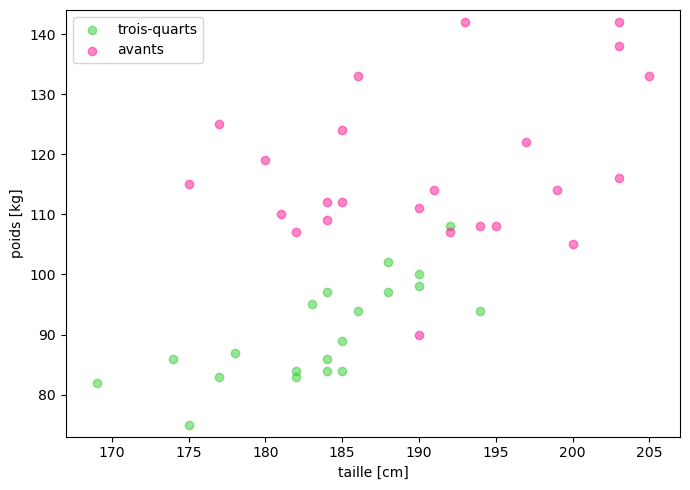
\includegraphics[width=1.0\linewidth]{Images/exemple_rugby_1}
				\label{fig:exemple_rugby_1}
			\end{figure}			
		\end{column}
		\begin{column}{0.5\textwidth}
			Dans le tracé ci-contre:
			\begin{itemize}
				\item On voit que les avants sont à la fois plus grands et plus lourds.
				\item \`A quelques exceptions près, on pourrait avoir un problème linéairement séparable.
			\end{itemize}
		\end{column}
	\end{columns}	
\end{frame}

\begin{frame}{Exemple avec les joueurs de rugby}
	\begin{columns}
		\begin{column}{0.6\textwidth}
			\begin{figure}
				\centering
				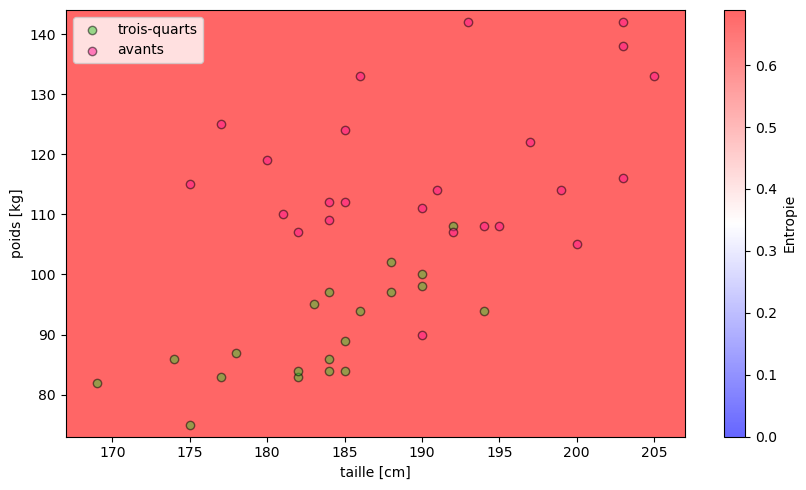
\includegraphics[width=1.0\linewidth]{Images/exemple_rugby_2}
				\label{fig:exemple_rugby_2}
			\end{figure}			
		\end{column}
		\begin{column}{0.4\textwidth}
			Ceci représente l'entropie de notre jeu de données avant que l'arbre de décision ne vienne \textbf{découper} les régions.
		\end{column}
	\end{columns}	
\end{frame}

\begin{frame}{Exemple avec les joueurs de rugby}
	\begin{columns}
		\begin{column}{0.6\textwidth}
			\begin{figure}
				\centering
				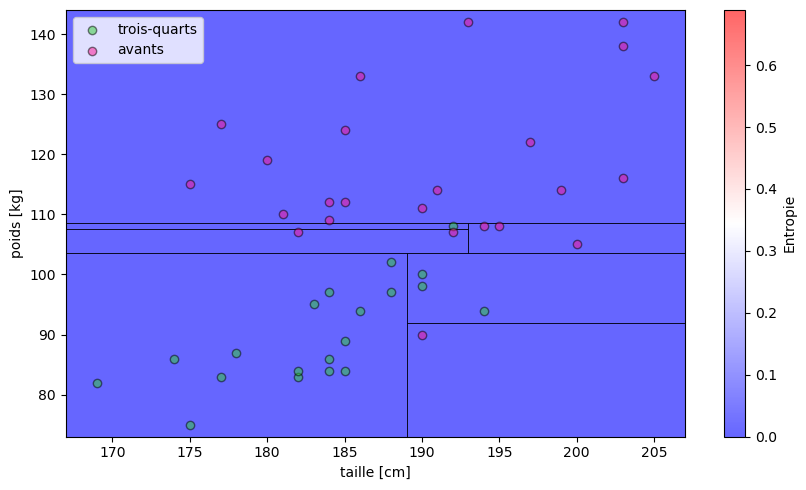
\includegraphics[width=1.0\linewidth]{Images/exemple_rugby_3}
				\label{fig:exemple_rugby_3}
			\end{figure}			
		\end{column}
		\begin{column}{0.4\textwidth}
			Après les découpes réalisées par l'arbre, on voit maintenant que chaque région a une entropie nulle. C'est parce que chaque région ne comporte soit que des avants, soit que des trois-quarts.
		\end{column}
	\end{columns}	
\end{frame}

\begin{frame}{Exemple avec les joueurs de rugby}
	\begin{columns}
		\begin{column}{0.6\textwidth}
			\begin{figure}
				\centering
				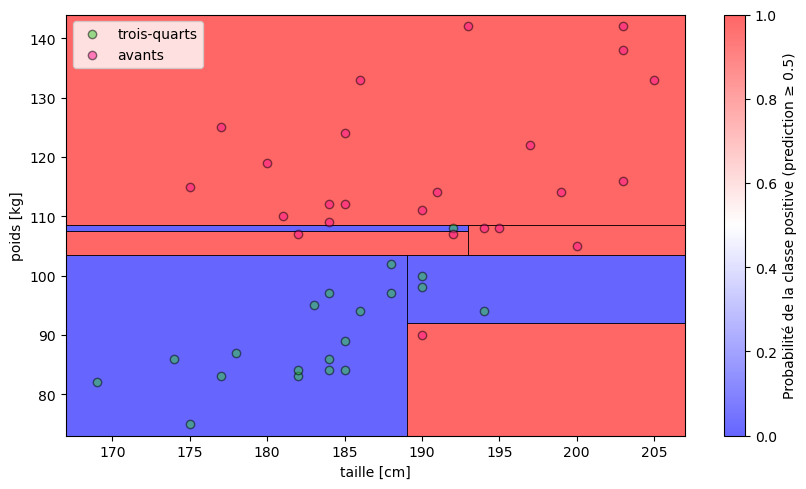
\includegraphics[width=1.0\linewidth]{Images/exemple_rugby_4}
				\label{fig:exemple_rugby_4}
			\end{figure}			
		\end{column}
		\begin{column}{0.4\textwidth}
			On représente ici la décision de l'arbre (en prenant comme hypothèse un seuil de décision $\theta = 0.5$). Comme chaque région a une entropie nulle, la prédiction donne soit une probabilité de 0, soit une probabilité de 1.
		\end{column}
	\end{columns}	
\end{frame}

\begin{frame}{Un second exemple}
	Dans ce second exemple on voit comment les zones découpées qui ont une entropie faible sont associées à des zones où les probabilités sont très tranchées (0 ou 1). \`A l'inverse, les régions conservant une entropie élevée sont associées à des probabilités moyennes.
	\begin{columns}
		\begin{column}{0.5\textwidth}
			\begin{figure}
				\centering
				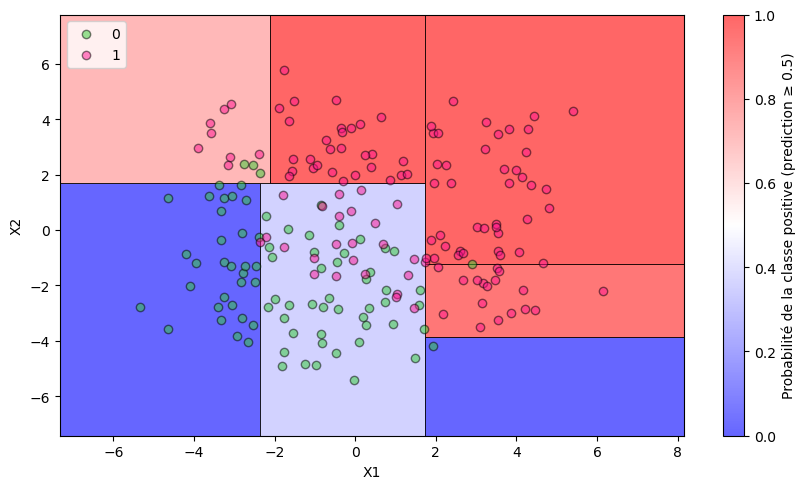
\includegraphics[width=1.0\linewidth]{Images/exemple_jouet_1}
				\label{fig:exemple_jouet_1}
			\end{figure}			
		\end{column}
		\begin{column}{0.5\textwidth}
			\begin{figure}
				\centering
				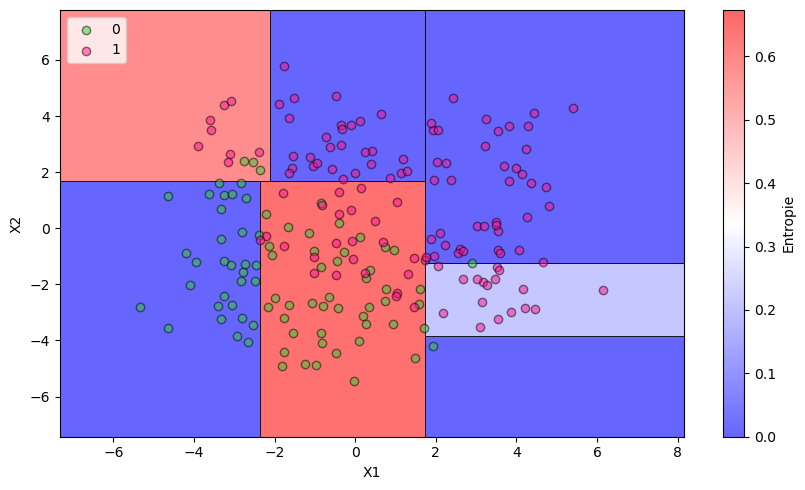
\includegraphics[width=1.0\linewidth]{Images/exemple_jouet_2}
				\label{fig:exemple_jouet_2}
			\end{figure}			
		\end{column}
	\end{columns}	
\end{frame}

\begin{frame}{Un second exemple}
	On peut régler les critères d'arrêts (profondeur, taille minimum, entropie minimum) pour obtenir un découpage \textit{parfait} sur les données d'apprentissage:
	\begin{columns}
		\begin{column}{0.5\textwidth}
			\begin{figure}
				\centering
				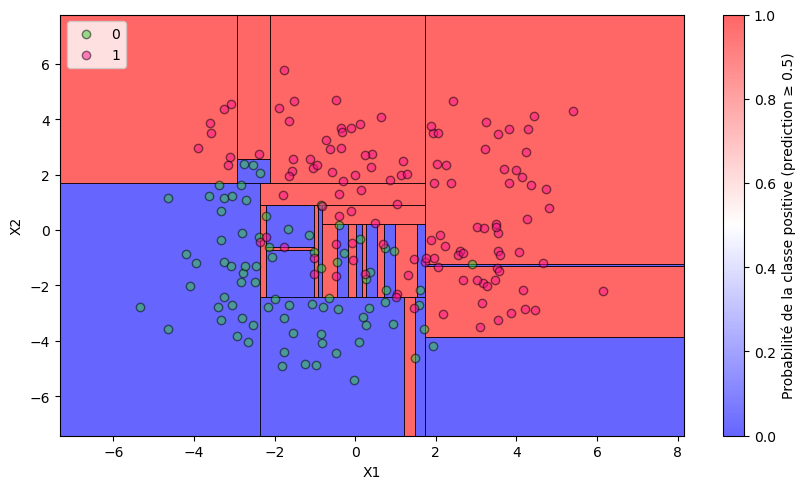
\includegraphics[width=1.0\linewidth]{Images/exemple_jouet_3}
				\label{fig:exemple_jouet_3}
			\end{figure}			
		\end{column}
		\begin{column}{0.5\textwidth}
			\begin{figure}
				\centering
				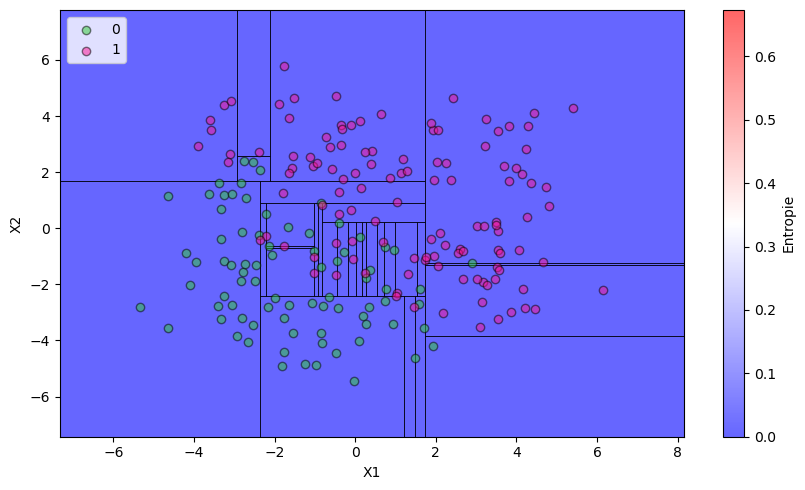
\includegraphics[width=1.0\linewidth]{Images/exemple_jouet_4}
				\label{fig:exemple_jouet_4}
			\end{figure}			
		\end{column}
	\end{columns}	
\end{frame}

\begin{frame}{Compromis biais / variance}
	\begin{itemize}
		\item Un découpage \textit{parfait} sur les données d'apprentissage ne garantit pas un découpage \textit{parfait} sur des données de test.
		\pause
		\item Un réglage trop agressif des critères d'arrêt peut conduire l'algorithme à du \textbf{sur-apprentissage}.
		\pause
		\item Dans un arbre de décision, le compromis sur le biais (sous-apprentissage) et la variance (sur-apprentissage) se fait sur la base des critères d'arrêt:
		\begin{itemize}
			\item \textbf{Taille minimum d'une feuille}: une valeur élevée introduit du biais et une valeur faible de la variance.
			\item \textbf{Entropie minimum}: une valeur élevée introduit du biais et une valeur faible de la variance.
			\item \textbf{Profondeur maximum}: une valeur faible introduit du biais et une valeur élevée de la variance.
		\end{itemize}
	\end{itemize}
\end{frame}